\begin{figure}[t]
\centering
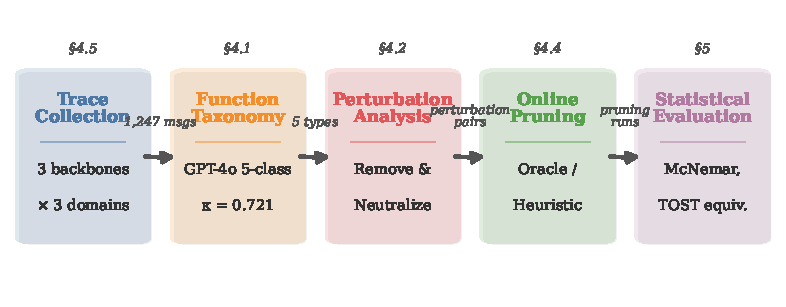
\includegraphics[width=\columnwidth]{figures/fig_pipeline.pdf}
\caption{Experimental pipeline. Multi-agent conversations (2{+}1 backbones $\times$ 3 domains, 15 configurations) are annotated into a 5-class taxonomy (cross-model $\kappa{=}0.721$), subjected to single-message perturbation analysis (remove and neutralize ablation), then pruned online under oracle or heuristic detection, and evaluated via McNemar exact tests and TOST equivalence.}
\label{fig:pipeline}
\end{figure}

\subsection{Analysis Protocol Overview}
\label{sec:framework_overview}

Existing MAS communication analyses operate at the turn level (which agent speaks when) or the system level (total token count). Neither captures the functional heterogeneity \emph{within} turns: a single checker response may acknowledge, verify, and redirect in successive sentences. We therefore adopt message-level granularity, classifying each message by its communicative function rather than its surface form.

The 5-class taxonomy---acknowledgment, verification, reasoning guidance, information provision, coordination---is derived from speech act theory~\cite{searle_speech_acts_1969} and conversation analysis~\cite{schegloff_discourse_1982, jefferson_acknowledgment_1984}, adapted to the structured interactions of LLM solver-checker systems. Five classes balance expressiveness against annotator reliability: coarser schemes (ack vs.\ non-ack) lose the impact gradient; finer schemes degrade inter-annotator agreement below actionable thresholds. The analysis protocol is designed for reuse: researchers can apply the taxonomy schema, annotation protocol, and statistical evaluation pipeline to any LLM-based multi-agent system without redesigning the classification or assessment methodology.

\subsection{Annotation Protocol}
\label{sec:taxonomy_method}

The annotation protocol is designed for reproducibility and portability across MAS configurations. Using the taxonomy from Section~\ref{sec:taxonomy}, each message is annotated via structured prompt with taxonomy definitions and hierarchical decision rules (temperature~0, constrained JSON output). To avoid self-annotation bias, messages generated by backbone $A$ are annotated by backbone $B$. Non-blinding could inflate ack classifications but makes the pruning test more conservative. The protocol requires only a taxonomy-aware LLM annotator and constrained decoding---no task-specific training data---making it directly applicable to new backbone or domain configurations. Our core claims depend on the ack/non-ack binary distinction (Cohen's $\kappa{=}0.721$~\cite{cohen_1960}, substantial agreement); fine-grained per-type agreement varies ($\kappa > 0.8$ for acknowledgment, $\kappa{=}0.237$ for information\_provision), so sub-category analyses are labeled preliminary. A human validation study ($N = 225$, $\kappa = 0.76$) is reported in Section~\ref{sec:discussion}.

\subsection{Perturbation-Based Impact Measurement}
\label{sec:perturbation}

To isolate each message's contribution to downstream behavior, we introduce two complementary ablation procedures applied independently to every message in a recorded conversation trace.

\paragraph{Remove ablation.} Message $m_i$ is deleted from trace $\mathcal{T}$, and all subsequent messages are discarded and regenerated from position $i+1$ onward. The behavioral impact is:
\begin{equation}
    \text{sim}_{\text{remove}}(m_i) = \cos\bigl(\mathbf{e}(a_{\text{orig}}),\, \mathbf{e}(a_{\text{regen}})\bigr)
\label{eq:impact}
\end{equation}
where $a_{\text{orig}}$ denotes the final solver answer in the original trace and $a_{\text{regen}}$ the answer regenerated from position $i{+}1$ after removing $m_i$; $\mathbf{e}(\cdot)$ denotes the sentence embedding from \texttt{all-MiniLM-L6-v2}~\cite{reimers_sentence_bert_2019}. Cosine similarity measures perturbation sensitivity---behavioral disruption from message removal. This is distinct from pruning safety, which is independently evaluated via task accuracy and McNemar's exact test (\S\ref{sec:pruning_protocol}, Table~\ref{tab:online_pruning}). The impact gradient (\S\ref{sec:impact_gradient}) characterizes perturbation patterns; it does not serve as the basis for pruning safety claims.

\paragraph{Neutralize ablation.} Message $m_i$ is replaced with a type-matched placeholder that preserves structural position while removing informational content. Comparing remove and neutralize ablation disentangles a message's \emph{content} from its \emph{structural presence}.

Each ablation is a single-message perturbation using greedy decoding via vLLM~\cite{kwon_vllm_2023} on 4$\times$ NVIDIA RTX PRO 6000 Blackwell Server Edition GPUs (96\,GB each), with conversations limited to $K = 6$ rounds.

\paragraph{Operational definitions.} \emph{Perturbation sensitivity}: $1 - \text{sim}_{\text{remove}}(m_i)$ (Eq.~\ref{eq:impact}). \emph{Informational importance}: task-relevant content operationalized via bigram novelty, token length, error correction rate, and Jaccard overlap.

\subsection{Statistical Framework}
\label{sec:statistical_framework}

The evaluation pipeline generalizes beyond acknowledgment pruning: any message-level intervention in a multi-agent system can be assessed by (1)~measuring per-type perturbation sensitivity via single-message ablation, (2)~testing aggregate pruning safety via McNemar's exact test and non-inferiority bounds, and (3)~quantifying equivalence via TOST. We instantiate this pipeline as follows.

We use OLS ANCOVA (Equation~\ref{eq:ols}) with function type as the factor and position/round as covariates, plus linear mixed-effects (ME) models (Equation~\ref{eq:me}) with task as a random intercept (the maximal converging specification):
\begin{equation}
    y_i = \beta_0 + \textstyle\sum_{k} \beta_k \cdot \text{FT}_{ik} + \gamma_1 \cdot \text{Pos}_i + \gamma_2 \cdot \text{Round}_i + \epsilon_i
\label{eq:ols}
\end{equation}
\begin{equation}
    y_{ij} = \beta_0 + \textstyle\sum_{k} \beta_k \cdot \text{FT}_{ijk} + \gamma_1 \cdot \text{Pos}_{ij} + \gamma_2 \cdot \text{Round}_{ij} + u_j + \epsilon_{ij}
\label{eq:me}
\end{equation}
where $u_j \sim \mathcal{N}(0, \sigma^2_u)$. Per-configuration ME models use individual tasks as random intercepts (maximal converging specification). Function type significance is tested via LRT with Benjamini--Hochberg correction ($\alpha = 0.05$; nine primary tests). End-to-end pruning safety is assessed primarily via confidence intervals on accuracy deltas (e.g., Qwen oracle 10-seed 95\% CI $[-0.33, +1.13]$\,pp) and McNemar's exact test~\cite{mcnemar_1947}. Non-inferiority testing at $\delta = -3$\,pp provides supplementary evidence: at baseline ${\sim}90\%$, this margin represents a ${\sim}30\%$ relative increase in error rate ($10\% \to 13\%$), calibrated against observed seed-to-seed variance ($\text{SD} \approx 1$--$2.4$\,pp) to separate genuine degradation from sampling noise (Appendix~\ref{app:margin_selection})~\cite{lakens_equivalence_2017}. TOST equivalence at $\pm 1$\,pp further quantifies precision where applicable (Qwen oracle $p = 0.048$, marginal; interpret alongside the CI).

\paragraph{Multiple comparison framework.} We organize statistical tests into three families to control false discovery risk while preserving power. \emph{Family~A} (primary confirmatory): nine LRT tests for function-type effects in mixed-effects models receive Benjamini--Hochberg correction at $\alpha = 0.05$. \emph{Family~B} (online cross-domain): McNemar tests across the backbone$\times$domain pruning matrix receive BH correction within family. \emph{Family~C} (offline exploratory): single-run offline comparisons (e.g., FG vs.\ ack-only, $N{=}100$) are explicitly labeled exploratory and do not receive cross-family correction. This hierarchy follows the confirmatory/exploratory distinction recommended in pre-registration practice; all Family~C $p$-values are reported for transparency but should not be interpreted as confirmatory evidence.

\subsection{End-to-End Pruning Protocol}
\label{sec:pruning_protocol}

We use \emph{pruning} to refer to three distinct operations: (1)~\emph{remove-one ablation}---removing a single message to measure local impact (\S\ref{sec:perturbation}); (2)~\emph{offline replay}---removing all messages of a given type and replaying the conversation; (3)~\emph{online suppression}---intercepting and withholding messages in real time during live agent interaction. Context disambiguates throughout.
Messages are suppressed per strategy and the conversation suffix is regenerated from the first suppression point. Four strategies are compared (\S\ref{sec:e2e_pruning}): Baseline, Ack-only, FG (lowest-impact function type), and Random (10 seeds). Each ``seed'' controls problem selection (greedy decoding is deterministic).

\paragraph{Oracle detection.} Two oracle pipelines establish upper bounds with perfect function-type detection. The \emph{offline} pipeline precomputes GPT-4o labels on baseline conversations; the \emph{online} pipeline annotates each message in real time within the pruned trajectory, eliminating distribution-shift confounds at higher cost. GPT-4o vs.\ GPT-4o-mini validation ($\kappa = 0.822$; Appendix~\ref{app:annotation_agreement}) confirms a cost-effective substitute.

\subsection{Heuristic Detector Development}
\label{sec:heuristic}

Because backbone choice determines communication surface form (\S\ref{sec:cross_domain}), we develop \emph{model-adapted} heuristic detectors that require no LLM annotation---analogous to task-specific prompt engineering, where rules are tuned to the target system rather than designed for universal transfer.

\paragraph{Qwen detector.} A character-length threshold ($< 30$) exploits Qwen's narrow ack surface band (42.2\% of checker messages below 30~chars, median 4~tokens; Appendix~\ref{app:info_theory}), yielding F1 $= 0.845$ on GSM8K with ${\sim}42\%$ suppression.

\paragraph{Llama detector.} Llama's verbose acks (mean 59.8~tokens, 65.6\% bigram novelty; Appendix~\ref{app:info_theory}) render length thresholds near-vacuous. A composite detector combines keyword matching, 4-gram repetition ratio ($> 0.3$), and a relaxed length ceiling ($< 300$~chars), yielding ${\sim}75\%$ suppression with comparable pruning safety (\S\ref{sec:e2e_pruning}).

Both detectors are task-specific proof-of-concept classifiers; limitations are evaluated in Section~\ref{sec:boundary} and discussed in Section~\ref{sec:discussion}.

\subsection{Learned Classification}
\label{sec:learned_classifier}

To quantify the gap between hand-crafted heuristics and learned detectors, we train supervised classifiers on the binary ack/non-ack label derived from the 5-class oracle annotations. The training corpus comprises 6{,}069 messages spanning all three backbones (Llama, Qwen, Gemma) and four domains (GSM8K, StrategyQA, ARC, MATH). We split by \texttt{task\_id} hash (70/20/10 train/val/test) to prevent messages from the same problem instance from appearing in both training and evaluation sets---a critical design choice, since messages within a task share surface cues that would inflate held-out scores under random splitting.

\paragraph{TF-IDF + logistic regression.} Character $n$-grams ($n{=}2$--$5$, \texttt{char\_wb}) and word $n$-grams ($n{=}1$--$2$) are extracted via TF-IDF and fed to a balanced logistic regression classifier. This lightweight pipeline achieves test-set F1~$= 0.859$ (macro-averaged, $N{=}526$), substantially outperforming the best heuristic detector (F1~$= 0.542$), confirming that learned features capture ack surface patterns that hand-crafted rules miss across backbone--domain combinations.

Fine-tuning DistilBERT~\cite{sanh_distilbert_2019} on the same split achieves test-set F1~$= 0.867$ (macro; ack-class $0.822$), comparable to TF-IDF+LR, confirming the lightweight pipeline as a practical alternative.

The cross-backbone, cross-domain training set ensures that classifiers generalize beyond any single configuration. Importantly, oracle pruning safety (\S\ref{sec:e2e_pruning}) does not depend on detector quality---it establishes an upper bound under perfect detection---so learned classifiers serve as practical deployment tools rather than prerequisites for the pruning result.

\subsection{Cross-Domain Experimental Design}
\label{sec:cross_domain_design}

A $3 \times 3$ factorial design (two primary backbones + one exploratory $\times$ three domains: GSM8K~\cite{cobbe_gsm8k_2021}, ARC-Challenge~\cite{clark_arc_2018}, StrategyQA~\cite{geva_strategyqa_2021}) yields 15 configurations (GSM8K under RR/SEQ/SEL; ARC and StratQA under RR only).
